\documentclass{article}

% Bitte hier die von Ihnen ben�tigten Style-Files laden
% Please load here the style files you need.
%\usepackage{german}
\usepackage{amsmath}
%\usepackage{graphics}
\usepackage{graphicx}
\newcommand{\mb}[1]{\ensuremath{\mbox{\boldmath $ #1 $}}}
\newcommand{\mbss}[1]{\ensuremath{\mbox{\boldmath $ \scriptstyle #1 $}}}
\newcommand{\av}[1]{\ensuremath{\langle #1 \rangle}}
\newcommand{\dubint}{\int\!\!\!\int}
\newcommand{\intZ}{\int\!\!\!\int}

\usepackage{oljour}

\begin{document}

% Bitte entfernen Sie das Kommentarzeichen vor dem K�rzel der
% Zeitschrift, in der Ihr Beitrag erscheinen soll.
% Please remove the comment char in the line that contains
% the shortcut for the journal where your submission shall
% appear

%\journalname{an}  % (analysis)
%\journalname{at}  % (Automatisierungstechnik)
%\journalname{it}  % (Information Technology)
%\journalname{ic}  % (icom)
%\journalname{rc}  % (Radiochimica Acta)
%\journalname{sd}  % (Statistics & Decisions)
%\journalname{tm}  % (Technisches Messen)
\journalname{zk}  % (Zeitschrift f�r Kristallographie)
%\journalname{zp}  % (ZPC)

% Titel des Beitrags (auf deutsch)
% Title of the submission (in german)
\title[de]{}

% Englischer Titel
% Title in english
\title[en]{Molecular Crystal Global Phase Diagrams II: Prototypical crystal packings for group T$_d$ molecules}

% Detaillierte Angaben zu allen Autoren des Beitrags:
% Bitte verwenden Sie f�r jeden Autor eine separate
% (begin/end) author-Umgebung.
% Detailed information about all authors of the submission:
% Please use for every author a separate
% (begin/end) author environment
\begin{author}
  \anumber{}   %fortlaufende Nummer (running number)
  \atitle{}    %akademischer Titel (academic title)
  \firstname{J. Brandon}  %Vorname(n) (first name(s))
  \surname{Keith}    %Nachname (surname)
  \vita{}      %Kurzlebenslauf (short curriculum vitae)
  \institute{Department of Chemical Engineering and Materials
Science, University of Minnesota, Minneapolis, Minnesota}   %Institutsname (name of institute)
  \street{Washington Avenue SE}    %Stra�e (street)
  \number{421}    %Hausnummer (number)
  \zip{55455}      %Postleitzahl (zip code)
  \country{Minneapolis MN, USA}   %Land (country)
  \tel{}      %Telefon (+COUNTRY-AREA-NUMBER: +49-341-49122701)
  \fax{}      %Fax
  \email{}     %E-Mail-Adresse (email address)
\end{author}

\begin{author}
  \anumber{}   %fortlaufende Nummer (running number)
  \atitle{}    %akademischer Titel (academic title)
  \firstname{Richard B.}  %Vorname(n) (first name(s))
  \surname{McClurg}    %Nachname (surname)
  \vita{}      %Kurzlebenslauf (short curriculum vitae)
  \institute{Department of Chemical Engineering and Materials
Science, University of Minnesota, Minneapolis, Minnesota}   %Institutsname (name of institute)
  \street{Washington Avenue SE}    %Stra�e (street)
  \number{421}    %Hausnummer (number)
  \zip{55455}      %Postleitzahl (zip code)
  \country{Minneapolis MN, USA}   %Land (country)
  \tel{}      %Telefon (+COUNTRY-AREA-NUMBER: +49-341-49122701)
  \fax{}      %Fax
  \email{}     %E-Mail-Adresse (email address)
\end{author}

% E-Mail-Adresse f�r die Korrespondenz des Verlags zu diesem
% Beitrag
% Corresponding address (for the publisher) for this submission
\corresponding{jbrkeith@gmail.com}

% englische Zusammenfassung des Beitrags
% english summary of the submission
\abstract{Previously~\cite{Keith04c,Mettes04}, we developed a method
for constructing global phase diagrams (GPDs) for molecular crystals
in which crystal structure is presented as a function of
intermolecular potential parameters. These diagrams are useful for
crystal design and reverse engineering the intermolecular potential
of an experimentally observed crystal structure. We apply this
method to fully ordered single component crystals composed of
tetrahedral molecules in the Cambridge Structural Database. In this
paper we find the number of molecular packings, called reference
lattices, to use in GPDs. We find the structures of these molecules
pack in 15 reference lattices: bcc (25.7\%), fcc (24.3\%), A5
(8.6\%), hcp (8.6\%), sc (8.6\%), and others (24.2\%).}

% deutsche Zusammenfassung des Beitrags
% german summary of the submission
\zusammenfassung{}

% bis zu sechs Keywords (englisch)
% up to six keywords (english)
\keywords{}

% bis zu sechs Schlagw�rter (deutsch)
% up to six keywords (german)
\schlagwort{}

% Widmung
% dedication
\dedication{}

% Die nachfolgenden Angaben werden in der Regel vom Verlag eingetragen.
% The following information is usually supplied by the publisher.
%======================================================================
\received{}
\accepted{}
\volume{}
\issue{}
\class{}
\Year{}
%======================================================================

\maketitle

% Hier bitte den Inhalt des Artikels einf�gen.
% Please insert the content of your submission here.
\section{Introduction}

Previously, we introduced a tool for exploring the molecular
parameter space of plastic and molecular crystals called a global
phase diagram (GPD)~\cite{Keith04c,Mettes04}. Global phase diagrams
summarize the phase behavior of a class of substances as a function
either of parameters in an empirical equation of state or of
parameters in an intermolecular potential. The classic example of a
GPD of the first type is the classification scheme for high pressure
vapor liquid phase equilibria by van
Konynenburg~\cite{VanKonynenburg80}. Their classification was based
on the van der Waals equation of state with simple binary mixing
rules. Despite the crude equation of state employed, it is still
widely used to classify the phase behavior of real binary mixtures.
Our GPD's are of the second type. They use an intermolecular
potential constructed from a complete set of basis functions for
rotational space for all molecules of a particular point group and a
set of molecular center-of-mass packings inferred from experimental
crystal structures. The parameters of the intermolecular potential
become axes on GPD's for each packing and the crystal structures are
phase regions in the diagrams.

An important benchmark of GPD's utility is to show that
experimentally observed structures can be found and their
intermolecular potential parameters can be read from the axes. Our
goal is to determine the number of translational packings, or
reference lattices, required in GPD construction and the number of
potential parameters needed to find all experimental phases.  A
small number of each will disprove previous hypotheses that many
parameters are needed~\cite{Briels80} and enhance the usability of
GPD's in materials design.

The outline of the balance of the paper is as follows. In
Sec.~\ref{Reference_Phases} we discuss the derivation of our data
set, its chemical and crystallographic characteristics, and group
entries based on structural similarity. In Sec.~\ref{assignments} we
deduce reference lattices for each structure by pseudo-symmetry
detection and describe the fit of the structures to these lattices.
Section~\ref{discussion} closes with a discussion of these results
and their application to GPDs, which is the subject of a subsequent
publication.~\cite{Keith06b}

\section{Experimental Data Set}
\label{Reference_Phases}

Since our molecular crystal global phase diagrams are constructed
for molecules of a given molecular point group symmetry, we have
chosen to use the \emph{CSDSymmetry} database as our primary source
of crystal structures~\cite{Yao02}. This database summarizes the
point groups of molecules that form error-free, nonpolymeric,
nonionic, coordinate-determined molecular crystals in the CSD.
Duplicates were removed from the database and hydrogen atoms were
not considered when assigning point groups. While the methods
introduced in our previous work~\cite{Mettes04} are applicable to
disordered structures, which are systematically absent from
\emph{CSDSymmetry}, it is a convenient source of crystal data for
molecules of a particular point group. Our methods are restricted to
single component crystals, however. Therefore we worked with the
single component crystal subset of the \emph{CSDSymmetry} database.
This was accomplished by first querying the CSD for all single
component crystals using {C\small ONQUEST}, the interface to the
CSD, and then using {C\small ONQUEST} to take the intersection of
the two data sets.

Continuing the example begun in our prior work~\cite{Mettes04}, we
chose to consider crystals composed of molecules with T$_d$
molecular point group symmetry.  We have augmented the data from
\emph{CSDSymmetry} with a recently determined structure of the low
temperature ordered phase of heavy methane~\cite{Neumann03}.  The
data set contains 71 crystal structures of 70 different chemical
substances.  Only carbon tetrachloride ($\mathrm{CCl}_4$) appeared
twice in different polymorphs. [CSD structures
CARBTC~\cite{Piermarini73} and CARBTC07~\cite{Cohen79}]. Names and
chemical formulas for all the entries are given in
Table~\ref{names1}. The chemical structures include 15 hydrocarbons
and their substituted derivatives and 56 organometallics. The
organometallics contain 30 different metals: Al, As, Bi, Cd, Co, Cs,
Cu, Ga, Ge, Hf, In, Mg, Mn, Na, Ni, Np, Pb, Pt, Re, Rh, Ru, Sb, Si,
Se, Sn, Tc, Th, Ti, U, and Zn. Eight types of molecular frameworks
are present in the data set: Cubane (29), Adamantane (17), MX$_4$
(16), Tetrahedrane (3), and others (6). There are entries from all
seven crystal systems in the data set. Twenty crystals are cubic (or
isometric), one is hexagonal, five are trigonal, ten are tetragonal,
six are orthorhombic, 22 are monoclinic, and seven are triclinic as
shown in Fig.~\ref{distro}. This distribution is different than the
CSD as a whole~\cite{Bauer92}, but that is not surprising given the
larger-than-average number of symmetries in the T$_d$ point group.
The data set is sufficient however to test whether molecular crystal
global phase diagrams apply to hydrocarbons and organometallics, a
variety of molecular frameworks, and all seven crystal systems.

One entry [CSD structure XUWROW~\cite{sung02}] is a very unusual
structure containing 70\% voids as recorded by the CCDC staff in its
cif file in the CSD, presumably using the standard van der Waals
radii in the documentation of CCDC software~\cite{Bruno02}. It was
grown as a thin epitaxial crystal under ultra-high vacuum.
Apparently the crystal structure is strongly influenced by the
substrate and we exclude it from further consideration.

The remaining crystal structures were organized into groups that
bear a strong ``structural relation'' as discussed in the
International Tables for Crystallography (ITC)~\cite{Hahn83}. For
crystals to belong to the same group they must have the same space
group symmetry, cell lengths in similar proportions, similar cell
angles, and molecular centers at equivalent Wyckoff point(s) with
similar structural parameter values where applicable.  We refer to
these groups as sharing a particular distinct structure. Note that
we do not require that the atomic positions be similar to be
classified in the same distinct structure. For example, two
structures [CSD structures DILWIE01~\cite{Ebert98} and
ZEYHIU~\cite{Noth95}] crystallize in space group 165 with molecules
at Wyckoff point d. Their cell parameters are also in similar
ratios. Therefore, we classify them in the same distinct structure,
despite their different chemical structures with different numbers
of atoms.

Two structures in \emph{CSDSymmetry} [CSD structures
HMGETP~\cite{Dahl75} and JUFWUC~\cite{Tesh92}] have molecules that
are tetrahedral within the default error bounds for detecting
molecular symmetry, but are sufficiently distorted to influence
their space group classifications (195a and 197a, respectively).
Either the molecules are very slightly distorted in the crystal or
the crystal symmetries are under-specified and actually belong to
space groups 215 and 217, respectively. Although slight distortions
could result from crystal Jahn-Teller distortions, for example, we
adopt the later interpretation. Therefore these crystals have been
grouped with distinct structures 215a and 217a, respectively. This
assignment is discussed from an energetic point of view in
Ref.~\cite{Keith06b}.

The 70 crystal structures fell into 46 distinct structures. Five
structures are cubic (or isometric), one is hexagonal, four are
trigonal, eight are tetragonal, six are orthorhombic, sixteen are
monoclinic, and six are triclinic. These distinct structures are
further characterized in the following section.

\section{Reference Lattice Assignments}
\label{assignments}

Our global phase diagrams are constructed starting with a fully
disordered plastically crystalline reference state.  At sufficiently
high temperature the intermolecular potential, which hinders free
rotation, becomes weaker than the thermal energy.  In this limit
molecules are free to disorder and ultimately to freely rotate.
Since the molecules are disordered they may occupy high symmetry
Wyckoff points in high symmetry space groups. These are space groups
with special values of the cell parameters
$(a,b,c,\alpha,\beta,\gamma)$ and molecules located at special
values of the unit cell fractional coordinates (x,y,z). Each
molecule has four or more generally equivalent non-coplanar nearest
neighbors. This is needed for structural stability in three
dimensions. We call these reference lattices.

High symmetry reference lattices may be determined for an
experimental crystal structure by determining the space group formed
from the lattice of the molecular centers of mass. These
calculations were done using F{\small INDSYM} in the I{\small
SOTROPY} software suite~\cite{Stokes02b} with coordinates scaled by
the minimum unit cell length $\{a,b,c\}$ and a large error tolerance
setting (0.1). Initially it may seem unexpected that molecular
crystals, the majority of which belong to monoclinic or triclinic
space groups~\cite{Bassoul00}, should be slight distortions of high
symmetry lattices. However, prior work in this area has shown this
is not only possible but quite
common~\cite{Motherwell97,Reichling00}. Standard unit cell choices
for low symmetry crystals systems often hide the similarity of a
suitably-chosen supercell to a reference lattice in a higher
symmetry crystal system. This high translational symmetry is a
result of the close-packing tendency of molecules. Broken symmetries
are due to orientational ordering and anisotropic intermolecular
potentials.

Occasionally a structure arises with fewer than four nearest
neighbors per molecule.  Due to the inherent lack of structural
stability of this arrangement, this suggests the crystal is in fact
a lattice of molecular clusters, typically \emph{dimers}, acting as
a single entity.  In such a case the center of mass of the dimers is
used in F{\small INDSYM} again with a larger error tolerance.

Given a list of common reference lattices, we developed an automated
technique to identify the reference lattices of experimental
structures. From a list of possible reference lattices, we
superimpose an experimental structure on each possible lattice so
one molecule in each structure overlaps. Then the experimental
structure is rotated and isotropically scaled in order to minimize
the sum of the absolute values between the center of each molecule
of the experimental structure and the center of the closest
reference lattice molecule,
\begin{equation}
\min_{a,\mbss{\omega}}\sum_m|\mb{R}(a,\mb{\omega})\cdot\mb{X}^{\mathrm{exp}}_m
 - \mb{X}^{\mathrm{ref}}_{\mathrm{closest}}|,
\end{equation}
where $\mb{R}(a,\mb{\omega})$ is a Cartesian rotation matrix
multiplied by an isotropic scaling factor $a$
(Appendix~\ref{cartRot}), $\mb{X}^{\mathrm{exp}}_m$ is the center of
mass of a molecule in the experimental structure,
$\mb{X}^{\mathrm{ref}}_{\mathrm{closest}}$ is the center of mass of
the closest molecule in one of the possible reference lattices, and
$m$ sums over all molecules in the experimental structure, which is
typically limited to the first 14 neighbors of the superimposed
center molecule.  This cutoff is justified by CSD
studies~\cite{Peresypkina00} showing 14 to be the most common
molecular coordination number. This technique was used in a computer
program to identify the majority of the fcc, bcc, hcp, sc, and
diamond reference lattices.

Applying these techniques to our data set gives the reference
lattice assignments in Tables~\ref{cubic}-~\ref{mono}. Generally we
name reference lattices first by their common name (\emph{i.e.} fcc)
if available, then by their Strukturbericht designation (\emph{i.e.}
A15) if available, and then by their space group/filled Wyckoff
positions if necessary (\emph{i.e.} 70a).  The raw atomic positions,
symmetry operators, etc. contained in the cif and fdat data files
from the CSD were processed using the cctbx collection of
algorithms~\cite{Grosse-Kunstleve02}. Algorithms from the I{\small
SOTROPY} software suite~\cite{Stokes02b} and the Bilbao
Crystallographic Server~\cite{Kroumova03} were also used to identify
group-subgroup relations, track Wyckoff point evolution, etc. In the
following subsections we review the reference lattices for the
structures in the experimental data set.

\subsection{Cubic (Isometric) Space Groups}

The cubic crystal structures are summarized in Table~\ref{cubic}.
%Note that we use
%the space group designations of the 1983 version of ITC instead of
%the recent and less well-known edition~\cite{Hahn02}.
Each structure is listed as a space group number followed by its
occupied Wyckoff points. A representative of each structure is named
in the next column.  Under each representative structure is  the
reference lattice. In the third column is shown the ratio $|G|/Z$.
This is the number of symmetry operations $|G|$ per molecules in the
unit cell $Z$. We call this ratio the symmetry density of a crystal
structure. Defined in this way, the symmetry density is independent
of the choice of unit cells. For instance the primitive and
conventional fcc cells both have $|G|/Z=48$. The symmetry density is
a maximum of 48 for fcc, bcc, and sc sphere packings. Symmetry
breaking, by loss of a class of symmetry operations and/or loss of
translations, reduces the symmetry density. The index $[i]$ of a
group-subgroup relation is the ratio of $|G|/Z$ of the group and its
subgroup. Thus, the geometric interpretation of the index is the
amount by which the symmetry of the crystal is diluted by symmetry
breaking (ITC, p726)~\cite{Hahn83}. The number of entries bearing a
strong structural similarity to the representative is shown in the
fourth column. For example, structure 217a has space group 217 with
molecules situated at Wyckoff point a. Its representative is DEQPAQ
and in a disordered state the crystal has the bcc symmetry or
reference lattice. Its symmetry density is 24 and that of its
reference lattice 48. Therefore, its index in bcc is 2. There are 11
tetrahedral molecular crystals in \emph{CSDSymmetry} with this
structure.

The 20 crystal structures in Table~\ref{cubic} fall into five
distinct structural types listed in order of decreasing symmetry
density. Structure 227a is unique in that the Wyckoff point symmetry
in the reference lattice is consistent with $T_d$ molecular point
group symmetry. Therefore the (ordered) experimental structure has
the full symmetry of the (disordered) reference lattice. Structures
217a and 215a are subgroups of bcc and sc, both of index two. The
molecular symmetry ($T_d$) is a subgroup of the Wyckoff site
symmetry in the reference lattice ($O_h$). Thus the crystal symmetry
is reduced by molecular ordering. Structure 218a,c is similarly a
subgroup of index two of A15, but the molecules on the two occupied
Wyckoff sites are inequivalent, even in the reference lattice.  For
each of the preceding structures, there are no arbitrary cell
parameters or structural parameters. Thus the molecular centers of
mass coincide exactly with the reference lattice.

Structure 205c has one arbitrary parameter, $x$, for its occupied
Wyckoff point.  This is called a Wyckoff structural parameter.
Figure~\ref{fig:205c} shows the neighbor distances as a function of
the structural parameter. The representative experimental structure
[tetracarbonyl-nickel CSD structure FOJBUB02~\cite{Braga93}] has
molecules at Wyckoff point c with a structural parameter $x=0.122$
which is approximately midway between the sc limit ($x=1/4$) and a
doubly occupied fcc limit ($x=0$ or $1/2$). It is evident from the
figure that the crystal structure is equivalent for structural
parameters $x$ and $1/2-x$. Since the neighbor distances at the
experimental values of the structural parameter are qualitatively
different than in the sc lattice, the simple cubic reference lattice
is not acceptable for our purposes. The crystal is best viewed as a
dimer packing with dimer centers of mass on an fcc lattice as shown
in Fig.~\ref{dimers} for a dimer situated on the $(1/2,1/2,0)$ fcc
coordinate. Its three-fold axis is parallel to the body diagonal
direction. The dimer has point group symmetry $D_{3d}$ so we would
expect to identify this structure on a $D_{3d}$ global phase diagram
using an fcc reference lattice. This possibility is not pursued
further here.

\subsection{Hexagonal and Trigonal Space Groups}

The six structures with hexagonal or trigonal space groups fall into
five structural types summarized in Table~\ref{hex}.  The c/a ratio
is given for the experimental lattice in the third column. The c/a
ratio for the reference lattice is also given.  These are the ratios
of the experimental structure embedded in the reference lattice.
Thus c/a=1.22 for the bcc reference lattice row of the TCYMET
structure entry is not c/a of the bcc crystal but c/a of TCYMET
embedded in the bcc reference lattice. This embedding is shown in
Fig.\ \ref{bccEmbed} in which the lattice constant of the bcc
crystal, $a^\prime$, is compared to the lattice constants a and c of
TCYMET. In each case in Table~\ref{hex} the arbitrary parameters
differ by only a few percent from the ideal reference lattices. All
five reference lattices are sphere packings (hcp, bcc, or fcc).

In contrast to the cubic lattices, all of the hexagonal and trigonal
structures in the data set have molecules at Wyckoff points with
variable Wyckoff structural parameters, so their value is given in
the fourth column. Below these are shown the structural parameters
of the reference lattices.  Again the agreement between the
translational arrangements of molecules in a crystal with a
high-symmetry reference lattice is quite good.

\subsection{Tetragonal Space Groups}
\label{sec:tet}

Tetragonal structures are summarized in Table~\ref{tet}. We adopt
the unique c-axis orientation for tetragonal space groups. The ten
structures fall into eight structural types. Structure 142a contains
eight molecular centers in the unit cell.  Their molecular centers
differ by only 1\% from two conventional fcc cells stacked in the
z-direction.  The other structures are less trivially related to
their reference lattices and are tetragonally distorted to various
degrees.

With the exception of structure 142a, discussed above, each of the
tetragonal structures is a sub-group of structures 141a, 139a, or
123a. Figure \ref{fig:tetr} gives the neighbor distances for
tetragonal distortions of these lattices.  Note that there is a
tetragonal distortion that transforms fcc and bcc into one another.
As a result, structures 137b, 121a, 142a, 114a, and 88f could not be
uniquely assigned to a reference lattice solely based on their
group/sub-group relationships.  For these structures, the $c/a$
ratio provides the requisite additional information.  The
experimental $c/a$ ratios are marked with circles in
Fig.~\ref{fig:tetr}. There appear to be fewer than nine circles in
the figure because several of them overlap. Note that the
experimental structures cluster around the sphere packings (marked
with dashed lines) or distorted lattices with equidistant neighbors
(marked with dotted lines). For instance, the diamond lattice can be
tetragonally distorted to yield six equidistant second-nearest
neighbors (A5$^\prime$ in Fig.\ \ref{fig:tetr} for $c/a=2/\sqrt{7}$)
or eight equidistant nearest neighbors (A5$^{\prime\prime}$ in Fig.\
\ref{fig:tetr} for $c/a=2\sqrt{3}$). The Aa reference lattice is a
distorted bcc structure and has ten equidistant nearest neighbors
for $c/a=\sqrt{2/3}$. The A6 reference lattice at $c/a=\sqrt{6}$ is
a reference lattice for other molecules discussed in later sections.
Also there is an additional dimer structure, 88f, among them.

\subsection{Orthorhombic Space Groups}

Orthorhombic structures are summarized in Table~\ref{orth}. We have
adopted the C-centered setting for end centered unit cells. Each of
the six structures constitutes its own distinct structural type. Two
structures, 64d,f and 60c,d very nearly match the fcc and bcc
reference lattices respectively. Structure 19a is identified with
the 63c reference lattice which is an orthorhombic structure with 10
nearest neighbors and equal c and a lengths. The b/a=b/c ratio is
$\sqrt{5+2\sqrt{6}}$ and the structural parameter for Wyckoff point
c (0,y,1/4) is $y=(\sqrt{6}-1)/4$. The small discrepancies in the
19a $x$ and $y$ structural parameters in this case indicate that the
molecules have further relaxed from their reference lattice
locations.  The three structures in space group 62 provide
additional challenges, discussed below.

Whereas the structures in the data set from the higher crystal
classes are uniquely identified by their space group and Wyckoff
point(s), there are three distinct orthorhombic structures in space
group 62 with molecules at Wyckoff point c.  Therefore, 62c is
insufficient as an identifier for these structures.  Since there are
two arbitrary cell length parameters and two structural parameters
for 62c, it is impractical to plot the neighbor distances as a
function of
arbitrary parameters as in Fig.\ %\ref{fig:205c} and
\ref{fig:tetr}.  Instead we note that Wyckoff point c in space group
62 has four equivalent positions, two at $y=1/4$ and two at $y=3/4$.
Therefore we view the 3-dimensional structure as a set of layers in
the xz-plane uniformly stacked in the y-direction. Then the $c/a$
ratio and the structural parameters determine the symmetry of the
layers. CSD structure GUTCED~\cite{Dahl03} is composed of
alternating layers that are nearly on a square lattice. Based on the
stacking of these layers this is a slightly distorted fcc lattice.
CSD structure RIMMOP~\cite{Dahl03} has alternating rectangular
layers, which is more similar to the bcc reference lattice. The
layers in CSD structure JEYSEL are nearly hexagonal and stacked
vertically, rather than alternating. Therefore, it is associated
with the simple hexagonal (sh) reference lattice.  Thus the three
structures in space group 62 are associated with different reference
lattices.

\subsection{Monoclinic Space Groups}

Monoclinic structures are shown in Table~\ref{mono}. We adopt the
unique b-axis orientation, cell choice one, origin choice two, and C
centering for end centered lattices. All three lattice parameters
and one lattice angle are able to relax so we indicate the closeness
of the match for b/a, c/a, and $\beta$. The 22 structures fall into
16 distinct structural types. In dividing into these types it is
important to note that monoclinic space groups have multiple
nonstandard settings. Also, during symmetry breaking from a
high-symmetry parent phase to a monoclinic child phase, multiple
domains may form creating unit cells that at first examination
appear to be dissimilar.  An example is CSD structure REKYUB and CSD
structure BOGMEP.  In a standard setting the important unit cell
parameters are $(b/a,c/a,\beta)=(0.48,1.00,123)$ and
$(0.28,0.55,145)$, respectively. The molecular positions also appear
different. However, these are simply different domains of the same
symmetry-breaking pathway with equivalent unit cell specifications.
The phase transition is governed by the same IR, $L_3^-$, and order
parameter direction, P7, using the notation of Stokes and
Hatch~\cite{Stokes02b}. Thus we group them in the same structural
class.

Monoclinic structures have a greater diversity of reference lattices
although those of 9 of the 16 structures are still canonical sphere
packings. A good example of this hidden order in these low-symmetry
groups is 15f,f,f,f which has 32 molecules per unit cell and four
molecules per asymmetric unit, but still nearly packs in an fcc
lattice.

Many of the structures belong to the same space group but have
different spatial arrangements and so are grouped differently. This
is particularly apparent for space groups 14 and 15, two of the most
populous space groups in the CSD. A5$^\prime$, the distorted diamond
lattice, fits two of the monoclinic structures, and simple hexagonal
two more.  One new packing, 70, is an orthorhombic distorted diamond
lattice and has eight molecules at Wyckoff point a. The other new
packing, 136, is a tetragonal structure with dimers of molecules at
Wyckoff point f. Three additional dimer structures (TMSIAD, CAMPOV,
MXSNOX) have dimers centered at high symmetry Wykcoff points without
structural parameters.

\subsection{Triclinic Space Groups}

Triclinic structures are shown in Table~\ref{tri}. All lattice
parameters are variable and are listed.  The six structures fall in
seven distinct structural types with four reference lattices. There
are two new reference lattices. A6 is a tetragonal distortion of fcc
discussed in Sec.~\ref{sec:tet} and shown in Fig.~\ref{fig:tetr}. Ai
is a rhombohedral distortion intermediate between sc and bcc. Its
primitive cell a, b, and c parameters are all the same length and
$\cos(\alpha)=cos(\beta)=cos(\gamma)=-1/4$. Two dimer structures in
136 and Ai also exist, the latter with dimer complexes at a high
symmetry Wyckoff point so no structural parameters are listed in
Table~\ref{tri} for XAGXAE.

\subsection{Reference Lattice Summary}

The results of the reference lattice assignments of the experimental
structures are summarized in Table~\ref{summary}. The
Strukturbericht designation~\cite{Wilson51}, Pearson
symbol~\cite{Pearson67}, and common name are shown when known for
each reference lattice. The Strukturbericht designations beginning
with an A indicate the reference lattices are also the crystal
structures of various elements. The space group, occupied Wyckoff
positions, and percentage of experimental structures that pertain to
each lattice are also shown.

The fit of each experimental structure to its reference lattice is
summarized in Fig.~\ref{comparison}. In each box the experimental
lattice vectors, angles, or Wyckoff positions are compared with
their idealized values when inscribed in the corresponding reference
lattice. These figures are a visual summary of
Tables~\ref{cubic}-\ref{tri}. If the fit were perfect all data
points would lie directly on the line. The fit is quite good
indicating that most low symmetry molecular crystals have molecules
situated at or near lattice sites of high symmetry space groups. In
the inorganic crystal structure database (ICSD), which is largely
composed of atomic crystals, the most numerous structures are fcc,
bcc, hcp, etc.~\cite{Mighell80} Originally this was considered to be
distinct from the CSD which had primarily monoclinic and triclinic
structures. Figure \ref{comparison} challenges this distinction by
showing molecular centers of mass, however, are nearly situated on
lattice points of these archetypical high symmetry lattices so
prevalent in the ICSD. The comparative number of monomer and dimer
structures is shown in Fig.~\ref{dimerMonomer} as is the breakdown
of each into types of reference lattices. It is apparent that
although there are 15 reference lattices, 76\% of the structures are
well represented by only 5 reference lattices.

The dimer structures, reference lattices, and dimer complex point
group symmetries are listed in Table~\ref{tab:dimers}.  Such
structures can usually be identified by examining nearest neighbor
distances. The presence of three or fewer nearest neighbors is
evidence of dimerization. Many of the structures form $D_{3d}$ or
nearly $D_{3d}$ dimers as illustrated in Fig.~\ref{dimers}, the one
exception being CSD structure LUFYEQ~\cite{Wrackmeyer02} whose
molecules form $C_{2v}$ complexes.

With the three techniques we have introduced here, (1) dimer
screening by nearest neighbor inspection, (2) reference lattice
assignment by large tolerance molecular center symmetry
determination, (3) reference lattice recognition through template
matching, one may determine translational packings or reference
lattices for all structures in the CSD.  While the second step has
generally been done by hand, the first and third step have been
automated in Python and {M\small ATHEMATICA} scripts and are
available upon request.

\section{Discussion and Conclusion}
\label{discussion}

%\subsection{Reference Lattices}

We have shown that all of the single-component tetrahedral molecules
in the CSD can be related to a reference lattice, or a high-symmetry
starting point for GPD calculations.  These reference lattices are
generally high symmetry sphere packings or distortions thereof.
These results also show the centers of mass of molecular crystals
are not structurally distinct from atomic crystals, which also pack
in high symmetry sphere packings such as fcc, bcc, hcp, sc, and so
on~\cite{Mighell80}. From our experiences with tetrahedral molecules
we hypothesize that the prevalence of low symmetry space groups for
molecular crystals in the CSD~\cite{Allen02} is due to the
orientational ordering of molecules whose centers of mass are close
to the lattice points of a higher symmetry space group. This
reflects the close packing tendency of
molecules~\cite{Kitaigorodskii61}.

We have shown many structures in our data set can be related to
dimers situated on a high symmetry lattice. Understanding the
prevalence of dimer structures in the CSD is important when
designing configurational search algorithms for crystal structure
prediction. Also, since most crystal structures in our data set
belong to only a few translational packings, or reference lattices,
fewer GPD diagrams are necessary to describe crystallographic
structural space for a given point group of molecules.

%\subsection{Conclusions}

In conclusion, a molecular crystal global phase diagram (GPD) can
summarize the experimental data using a modest number of reference
lattices and IP parameters. In previous
work~\cite{Keith04c,Mettes04}, we somewhat arbitrarily chose a
single reference lattice (fcc) and truncated the intermolecular
potential with three terms to illustrate the method. Here, we have
used an experimental data set of crystals of tetrahedral molecules
to determine reference lattices and an IP truncation sufficient to
produce the observed phases. The data set is diverse enough to test
the GPD's ability to classify a wide range of space groups using a
common intermolecular potential. Just as the van Konynenburg global
phase diagram classification based on the simple van der Waals
equation of state is nonetheless widely used to classify the phase
behavior of real binary mixtures, molecular crystal global phase
diagrams may be useful in elucidating phase behavior of a variety of
real substances and, in turn, used to develop novel intermolecular
potentials and materials.

This work received financial support from the American Chemical
Society - Petroleum Research Fund (PRF \#41774-AC10).
%
Computational resources maintained by the University of Minnesota
Supercomputer Institute were used for portions of this research.

\appendix

\section{Cartesian Rotations}
\label{cartRot}

The cartesian rotation matrix,
\begin{eqnarray}
\mb{R}(a,\mb{\omega})=a\left(\begin{array}{c}\cos(\alpha)\cos(\beta)\cos(\gamma)
- \sin(\alpha))\sin(\gamma) \\
\cos(\beta)\cos(\gamma)\sin(\alpha) + \cos(\alpha)\sin(\gamma) \\
    -\cos(\gamma) \sin(\beta),\end{array} \right. \nonumber\\
%
\begin{array}{c}-\cos(\gamma)\sin(\alpha)-\cos(\alpha) \cos(\beta) \sin(\gamma)\\
\cos(\alpha)\cos(\gamma) - \cos(\beta)\sin(\alpha)\sin(\gamma) \\
    \sin(\beta) \sin(\gamma),\end{array} \nonumber\\
%
\left. \begin{array}{c}\cos(\alpha) \sin(\beta)\\
\sin(\alpha) \sin(\beta)\\
    \cos(\beta)\end{array}\right)
\end{eqnarray}
is produced by converting spherical coordinate Wigner functions to
cartesian coordinates.

\bibliography{thesisbib}

\begin{table}
\caption{Identifiers, chemical formulas, and assigned frameworks of
the tetrahedral data set.}\label{names1} \tiny
\begin{tabular}{lll}
Identifier & formula & framework\\
\hline
ADAMAN08 & C10 H16 & adamantane \\
BASXOI & C4 H12 Se6 Sn4 & adamantane \\
BOGMEP & C24 H48 Cl6 Cu4 N16 O1 & other \\
CAMPOV & C16 H36 N4 Sn4 & cubane\\
CANFIG & C4 H24 B4 U1 & MX$_4$\\
CANFOM & C4 H24 B4 Th1 & MX$_4$\\
CARBTC & C1 Cl4 & MX$_4$\\
CARBTC07 & C1 Cl4 & MX$_4$\\
CTBROM & C1 Br4 & MX$_4$\\
CUCZUV & C20 H36 & tetrahedrane\\
DEQPAQ & C36 H100 B4 N12 Na4 & other\\
DILWIE01 & C16 H48 Pt4 S4 & cubane\\
DOCNIS & C8 H12 S6 & adamantane\\
FOHCUA & C12 Ni4 O18 P4 & adamantane\\
FOJBUB02 & C4 Ni1 O4 & MX$_4$\\
FUZLUH & C12 Co4 O12 Sb4 & cubane\\
FUZTEZ & H16 B4 Np1 & MX$_4$\\
FUZVOL & H16 B4 Hf1 & MX$_4$\\
GERHOA & C4 H12 Cl12 N4 Sb4 & cubane\\
GUTCED & C26 H32 & other\\
HMGETP & C12 H36 Ge6 P4 & adamantane\\
HMSIPA & C12 H36 P4 Si6 & adamantane\\
HXMTAM07 & C6 H12 N4 & adamantane\\
JEYSEL & C18 H36 Ni4 O6 P4 & tetrahedrane\\
JUFWUC & C12 H40 Cs4 N4 Si4 & cubane\\
KANGUB01 & C10 H12 I4 & adamantane\\
KELREY & C12 H36 Cl4 Ti4 & cubane\\
KOXKOX & C16 H36 Ga4 Se4 & cubane\\
KUJSIR & C20 H48 O4 Zn4 & cubane\\
LUFYEQ & C12 H12 Si1 & MX$_4$\\
MECKIO & C16 H36 Cl4 In4 N4 & cubane\\
MECKOU & C16 H36 Br4 In4 N4 & cubane\\
MECKUA & C16 H36 I4 In4 N4 & cubane\\
MESIAD & C12 H36 As4 Si6 & adamantane\\
MEZDIE01 & C12 H36 Si1 Sn4 & MX$_4$\\
MEZDOK01 & C12 H36 Ge1 Sn4 & MX$_4$
\end{tabular}
\end{table}

\begin{table}
\caption{cont.}\tiny
\begin{tabular}{lll}
Identifier & formula & framework\\
\hline
MPTHOT01 & C12 H40 O4 Pt4 & cubane \\
MSISUL10 & C4 H12 S6 Si4 & adamantane\\
MTRETC10 & C16 H12 O12 Re4 S4 & cubane\\
MXSNOX & C4 H12 O8 Sn6 & other\\
MZNMOX10 & C8 H24 O4 Zn4 & cubane\\
NIWMIP & C12 H36 Al4 N4 S6 & adamantane\\
OHABEE & C16 H36 Si4 & tetrahedrane\\
POSLOY10 & C12 Cl4 O12 Tc4 & cubane\\
QUGBOJ & C16 O16 Rh6 & other\\
RASDOE & C16 H48 Ga4 N4 Si4 & cubane\\
REKYUB & C16 H36 Ga4 S4 & cubane\\
RIMMOP & C16 H40 Al4 N4 & cubane\\
RIMNAC & C20 H48 Al4 N4 & cubane\\
RUQMEV & C12 H36 Cu4 I4 N4 & cubane\\
SENLAY & C16 H36 P4 Si4 & cubane\\
TCYMET & C5 N4 & MX$_4$\\
TFMETH02 & C1 F4 & MX$_4$\\
TMEPTC & C12 H36 Cl4 Pt4 & cubane\\
TMGEHS10 & C4 H12 Ge4 S6 & adamantane\\
TMSIAD & C10 H24 Si4 & adamantane\\
TMSNHS10 & C4 H12 S6 Sn4 & adamantane\\
TOHSUE & C16 F12 O12 P4 Ru4 & cubane\\
VADRAU & C4 H12 Pb1 & MX$_4$\\
VAFWAA & C12 Bi4 Co4 O12 & cubane\\
VAVYAS & C20 H36 P4 & cubane\\
XAGXAE & P4 S10 & adamantane\\
XUWROW & C20 H48 Mg4 O4 & cubane\\
YEMRIR & O6 P4 S4 & adamantane\\
YEYQAU & C12 O12 Ru4 Se4 & cubane\\
YIMWEW & C10 H16 O4 & adamantane\\
ZEYHIU & C20 H48 Cd4 O4 & cubane\\
ZIZHIZ & C12 H4 Mn4 O16 & cubane\\
ZNOXAC01 & C12 H18 O13 Zn4 & other\\
ZZZKDW01 & C1 I4 & MX$_4$\\
\hline
\end{tabular}
\end{table}

\begin{figure}
\begin{center}
\scalebox{.7}{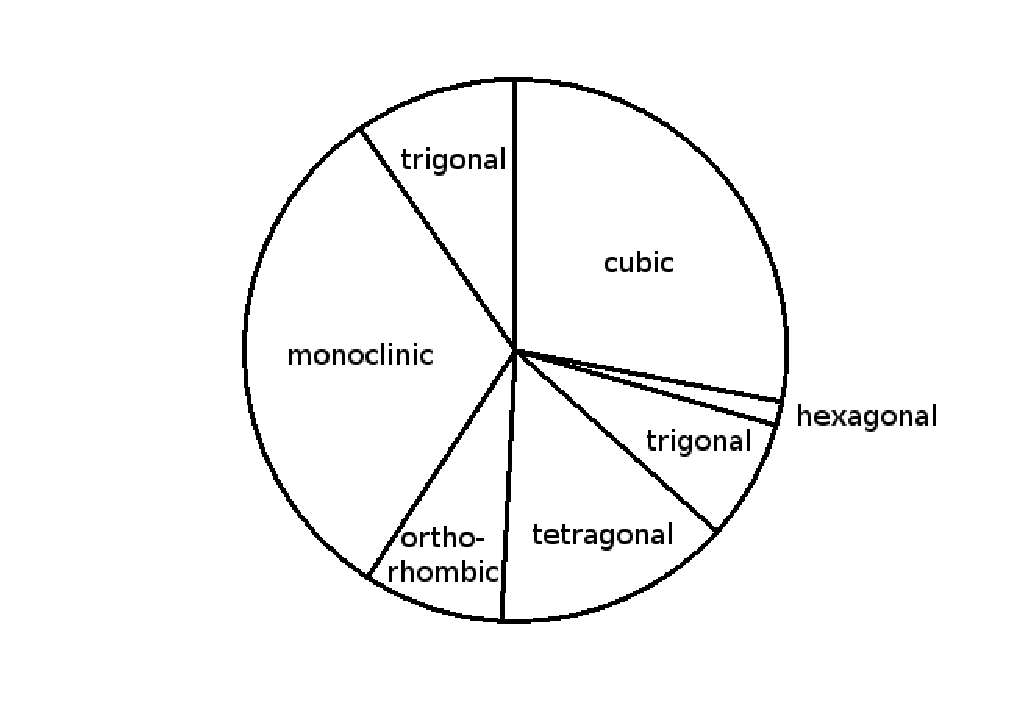
\includegraphics[width=\fullwidth]{crystalSystems.eps}}
%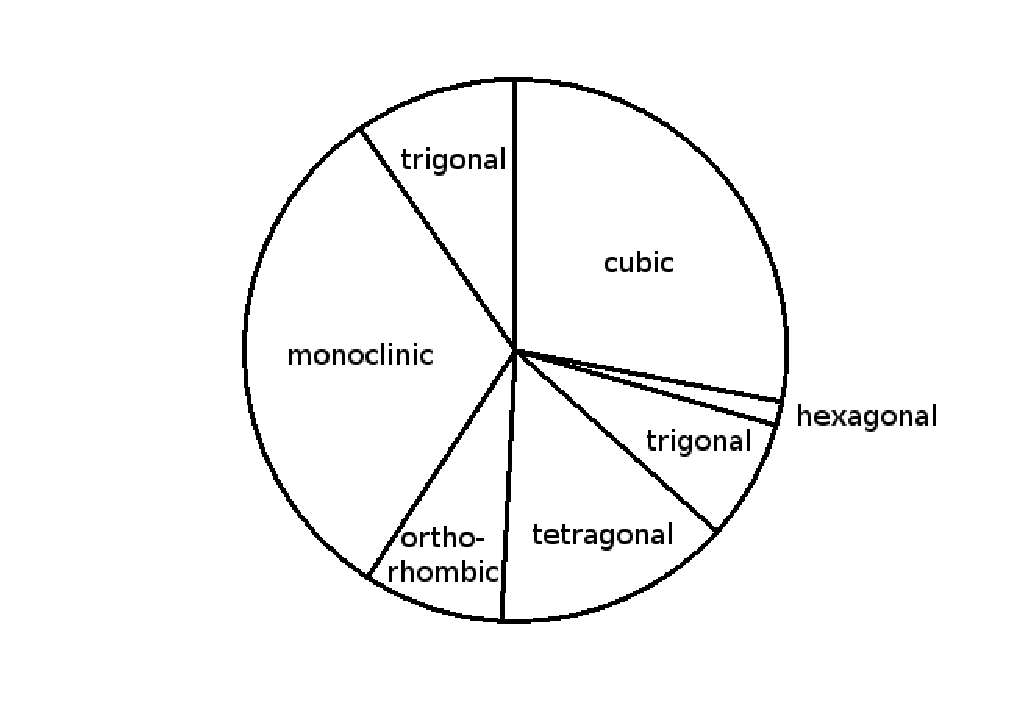
\includegraphics{crystalSystems.eps}
\caption[Distribution of experimental structures among the seven
crystal systems.]{Crystal systems for crystals of tetrahedral
molecules.\label{distro}}
\end{center}
\end{figure}

\begin{table}
\caption{Reference lattices for cubic (isometric) structures.}
\label{cubic}
\begin{center}
\begin{tabular}{cccc}%\hline
\cline{1-4}
Structure & Example & $|G|/Z$ & Entries \\
        & Lattice \\
\cline{1-4}
227a    & ZNOXAC01 & 24 & 1 \\
        & diam     & 24 \\
217a    & DEQPAQ   & 24 & 11 \\
        & bcc      & 48 \\
215a    & FOHCUA   & 24 & 3 \\
        & sc       & 48 \\
205c    & FOJBUB02 &  3 & 2 \\
        & d-fcc$^*$& 24 \\
218a,c  & SENLAY   &  3 & 3 \\
        & A15      &  6 \\
\cline{4-4}
\multicolumn{3}{r}{total:} & 20 \\
\cline{1-4}
\end{tabular} \\
$^*$ dimer packing
\end{center}
\end{table}

\begin{figure}
\begin{center}
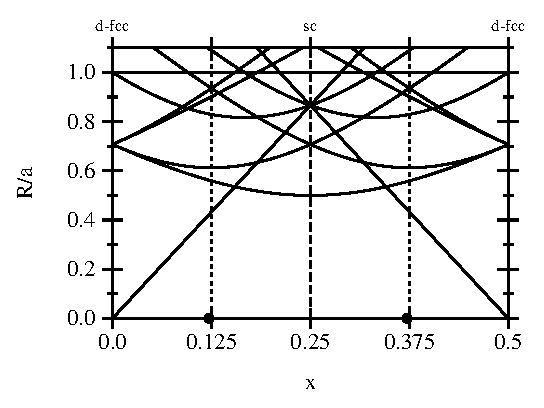
\includegraphics[width=\fullwidth]{205c.eps}
\end{center}
\caption[Neighbor distances for 205c as a function of $x$]{Neighbor
distances for 205c as a function of the Wyckoff structural
parameter, $x$.  The experimental structures, marked with circles,
are midway between the sc and doubly-occupied fcc limits.}
\label{fig:205c}
\end{figure}

\begin{figure}
\begin{center}
\scalebox{1}{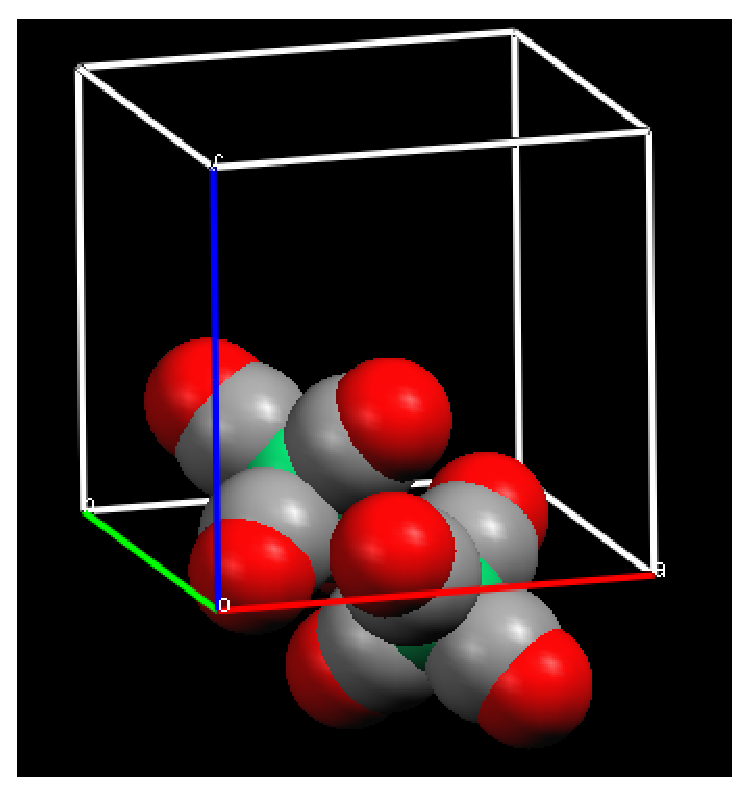
\includegraphics[width=\fullwidth]{FOJBUB02_Show.eps}}
%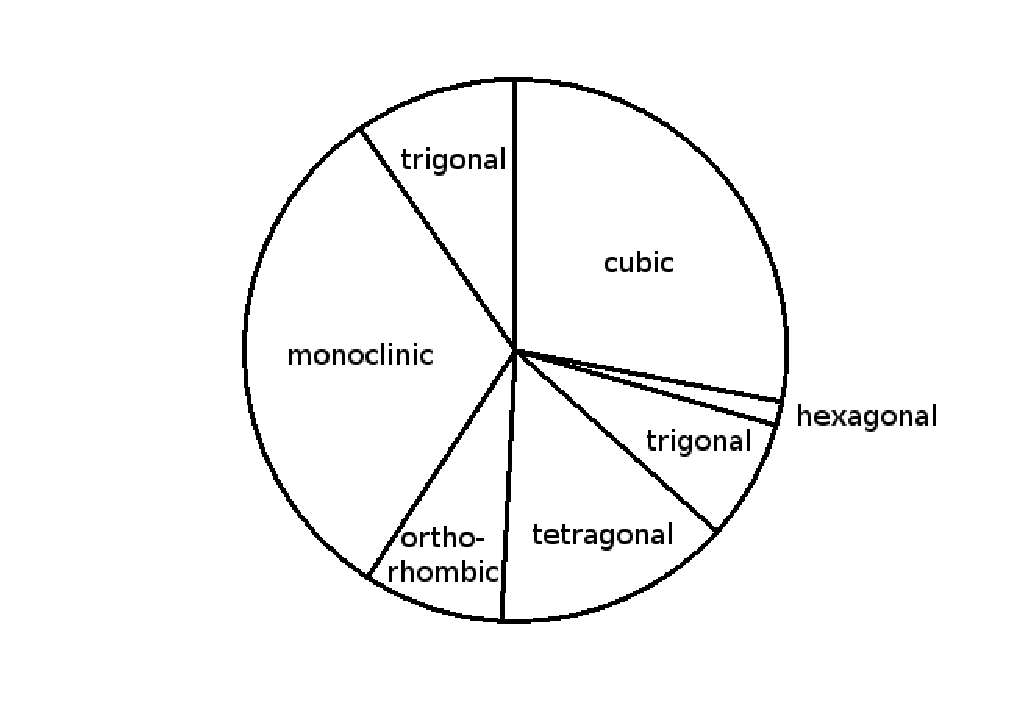
\includegraphics{crystalSystems.eps}
\caption[Crystal structure of tetracarbonyl-nickel in space group
205c]{Crystal structure of tetracarbonyl-nickel [CSD structure
FOJBUB02~\cite{Braga93}] in space group 205c with molecules at
Wyckoff point c. It is a fcc lattice of dimers at Wyckoff point a as
shown for one dimer centered at fractional coordinate
$(1/2,1/2,0)$.\label{dimers}}
\end{center}
\end{figure}

\begin{table}
\caption[Reference lattices for hexagonal and trigonal
structures.]{Reference lattices for hexagonal and trigonal
structures. Ideal reference lattice parameters and Wyckoff
structural parameters are listed below the experimental data.}
\label{hex}
\begin{center}
\begin{tabular}{cccccc}%\hline
\cline{1-6}
Structure & Example & c/a & Str.\ Param's & $|G|/Z$ & Entries \\
          & Lattice \\
\cline{1-6}
165d    & DILWIE01  & 3.07  & z=0.122          &  3 & 2 \\
        & hcp       & 3.27  & z=1/8            & 12 \\
161a    & TCYMET    & 1.28  & z=0.000          &  3 & 1 \\
        & bcc       & 1.22  & z=0              & 48 \\
147d    & ZIZHIZ    & 1.51  & z=0.252          &  3 & 1 \\
        & hcp       & 1.63  & z=1/4            & 12 \\
176h    & CUCZUV    & 0.89  & x=0.361, y=0.334 &  2 & 1 \\
        & hcp       & 0.94  & x=1/3, y=1/3     & 12 \\
152b    & MTRETC10  & 2.57  & x=0.715          &  2 & 1 \\
        & fcc       & 2.45  & x=2/3            & 48 \\
\cline{6-6}
\multicolumn{5}{r}{total:} & 6 \\
 \cline{1-6}
\end{tabular}
\end{center}
\end{table}

\begin{figure}
\begin{center}
\scalebox{1}{\includegraphics[width=\fullwidth]{tcymetSupercell_2.eps}}
\caption[The crystal structure of TCYMET embedded in a bcc reference
lattice.]{The crystal structure of TCYMET embedded in a bcc
reference lattice. The molecular centers of mass are depicted as
spheres. The lattice constant of the bcc reference lattice,
$a^\prime$, is compared to the lattice constants a and c of
TCYMET.\label{bccEmbed}}
\end{center}
\end{figure}

\begin{table}
\caption{Reference lattices for tetragonal structures} \label{tet}
\begin{center}
\begin{tabular}{cccccc}%\hline
\cline{1-6}
Structure & Example & c/a & Str.\ Parameters & $|G|/Z$ & Entries \\
          & Lattice \\
\cline{1-6}
141a    & FUZLUH    & 0.72 & & 8 & 2 \\
        & A5$^\prime$&0.76 & & 8 \\
137b    & FUZTEZ    & 0.70 & & 8 & 1 \\
        & Aa        & 0.82 & & 16 \\
121a    & ZZZKDW01  & 1.49 & & 8 & 1 \\
        & fcc       & 1.41 & & 48 \\
142a    & KUJSIR    & 2.02 & & 4 & 1 \\
        & fcc       & 2.00 & & 48 \\
120c    & YEMRIR    & 1.50 & & 4 & 1 \\
        & sc        & 1.41 & & 48 \\
114a    & ADAMAN08  & 1.34 & & 4 & 2 \\
        & fcc       & 1.41 & & 48 \\
88a     & KANGUB01  & 3.97 & & 4 & 1 \\
        & A5$^{\prime\prime}$& 3.46&&8 \\
88f     & LUFYEQ    & 1.25 & z=0.311&1&1 \\
        & d-Aa$*$     & 1.15 & z=3/8&8 \\
\cline{6-6}
\multicolumn{5}{r}{total:} & 10 \\
\cline{1-6}
\end{tabular} \\
$^*$ dimer packing
\end{center}
\end{table}

\begin{figure}
% \includegraphics{141ab.eps}
% \includegraphics{139ab.eps}
\begin{center}
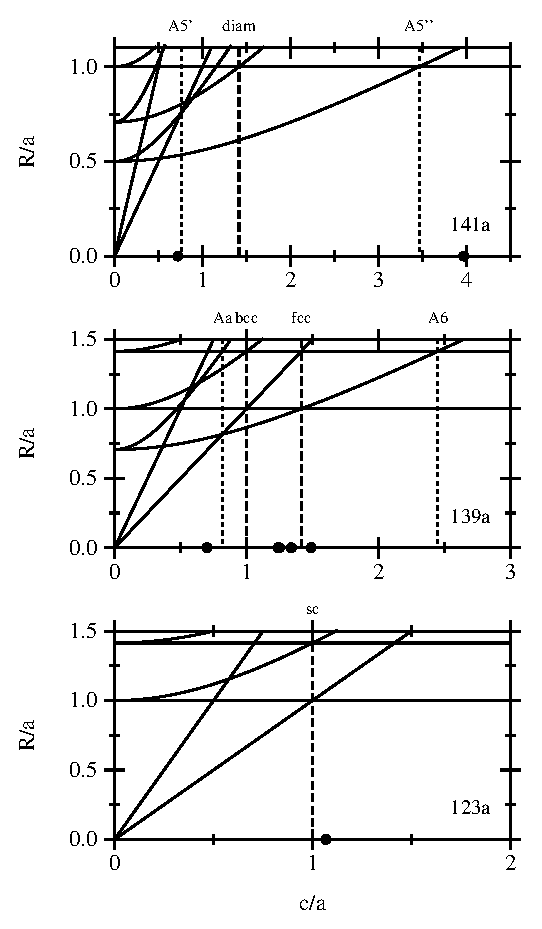
\includegraphics[width=\fullwidth]{tetrEPS.eps}
\end{center}
\caption[Neighbor distances for 141a, 139a, and 123a]{Neighbor
distances for 141a, 139a, and 123a as a function of the $c/a$ ratio.
The tetragonal distortions include diam, bcc, fcc, and sc as special
cases.  Experimental values are marked with circles.  Additional
neighbors are omitted for clarity at small $c/a$ values.}
\label{fig:tetr}
\end{figure}

\begin{table}
\caption{Reference lattices for orthorhombic structures}
\label{orth}
\begin{center}
\begin{tabular}{ccccccc}%\hline
\cline{1-7}
Structure & Example & b/a & c/a & Str.\ Parameters & $|G|/Z$ & Entries \\
          & Lattice \\
\cline{1-7}
62c     & GUTCED    & 1.10  & 1.09  & x=0.171, z=-0.014   & 2  & 1 \\
        & fcc       & 1.00  & 1.00  & x=1/4, z=0         & 48 \\
62c     & RIMMOP    & 1.46  & 1.61  & x=0.187, z=0.032   & 2  & 1 \\
        & bcc       & 1.41  & 1.41  & x=1/4, z=0         & 48 \\
62c     & JEYSEL    & 1.62  & 1.80  & x=-0.069, z=-0.030   & 2  & 1 \\
        & sh        & 1.63  & 1.73  & x=0, z=0           & 24 \\
64d,f   & METHANEIII& 0.70  & 0.70  & x=0.250            & 1  & 1 \\
        &           &       &       & y=0.230, z=0.270    \\
        & fcc       & 0.71  & 0.71  & x=1/4              & 48 \\
        &           &       &       & y=1/4, z=1/4 \\
19a     & MZNMOX10  & 1.03  & 3.93  & x=-0.066, y=0.067, z=0.123 & 1 & 1 \\
        & 63c       & 1.00  & 3.15  & x=0, y=0, z=0.112          & 4 \\
60c,d   & YIMWEW    & 0.45  & 0.46  & y=-0.188            & 2/3 & 1 \\
        &           &       &       & x=0.169, y=0.297, z=0.206 \\
        & bcc       & 0.47  & 0.47  & y=-1/4              & 48 & \\
        &           &       &       & x=1/6, y=1/4, z=1/4 \\
\cline{7-7}
\multicolumn{6}{r}{total:} & 6 \\
\cline{1-7}
\end{tabular}
\end{center}
\end{table}

\begin{table}
\caption{Reference lattices for monoclinic structures} \label{mono}
\begin{center}
\begin{tabular}{cccccccc}%\hline
\cline{1-8}
Structure & Example & b/a & c/a & $\beta$ & Str.\ Parameters & $|G|/Z$ & Entries \\
          & Lattice \\
\cline{1-8}
15e     & REKYUB    & 0.48 & 1.00 & 123 & y=-0.024 & 2 & 3 \\
        & fcc       & 0.58 & 1.16 & 125 & y=0   & 48 \\
15e     & RASDOE    & 0.51 & 0.97 & 120 & y=0.123 & 2 & 1 \\
        & 70a       & 0.50 & 1.00 & 120 & y=1/8   & 4 \\
15e     & TMGEHS10  & 1.78 & 1.14 & 108 & y=0.106 & 2 & 3 \\
        & A5$^\prime$& 1.87 & 1.06 & 118 & y=1/8   & 8 \\
12i     & MECKOU    & 0.73 & 1.17 & 110 & x=0.253, z=0.241 & 2 & 1 \\
        & fcc       & 0.58 & 1.00 & 109 & x=1/4, z=1/4     & 48 \\
11e     & MECKIO    & 1.61 & 1.13 & 105 & x=0.205, y=0.219 & 2 & 1 \\
        & bcc       & 1.63 & 1.00 & 109 & x=1/4, y=1/4     & 48 \\
14e     & TOHSUE    & 1.01 & 2.76 & 90  & x=0.250, y=0.745, z=0.126 & 1 & 1\\
        & fcc       & 1.00 & 2.83 & 90  & x=1/4, y=3/4, z=1/8       & 48 \\
14e     & TMSIAD    & 1.11 & 2.07 & 91  & & 1 & 1 \\
        & d-sh$*$  & 1.22 & 2.12 & 90  & & 12 \\
14e     & CAMPOV    & 1.41 & 1.64 & 92  & & 1 & 2 \\
        & d-sc$*$   & 1.41 & 1.41 & 90  & & 24 \\
14e     & DOCNIS    & 1.45 & 1.80 & 60  & x=0.102, y=0.255, z=0.072 & 1 & 1 \\
        & hcp       & 1.63 & 2.00 & 60  & x=1/6, y=1/4, z=1/12      & 12 \\
14e     & CARBTC    & 0.63 & 1.01 & 104 & x=0.248, y=0.067, z=0.157 & 1 & 1 \\
        & hcp       & 0.61 & 1.06 & 90  & x=1/4, y=0, z=1/6         & 12 \\
14e     & QUGBOJ    & 0.59 & 1.06 & 105 & x=0.268, y=0.129, z=0.070 & 1 & 1\\
        & A5$^\prime$&0.76 & 1.00 & 90  & x=1/4, y=1/8, z=0         & 8 \\
\cline{1-8}
\end{tabular}\\
$^*$ dimer packing
\end{center}
\end{table}

\begin{table}
\caption{cont.}
\begin{center}
\begin{tabular}{cccccccc}%\hline
\cline{1-8}
Structure & Example & b/a & c/a & $\beta$ & Str.\ Parameters & $|G|/Z$ & Entries \\
          & Lattice \\
\cline{1-8}
14e     & MECKUA    & 0.66 & 1.14 & 113 & x=0.501, y=0.225, z=0.749 & 1 & 1 \\
        & fcc       & 0.59 & 1.00 & 109 & x=1/2, y=1/4, z=3/4       & 48 \\
14e,e   & CANFIG    & 0.92 & 1.10 & 26  & x=0.331, y=0.340, z=0.005 & 1/2 & 1 \\
        & d-136$*$  & 1.00 & 1.12 & 27  & x=1/3, y=1/3, z=0         & 2 \\
14e,e   & MXSNOX    & 1.76 & 1.74 & 75  & & 1/2 & 1 \\
        & d-sh$*$   & 1.73 & 1.91 & 59  & & 12 \\
13e,f,g & RIMNAC    & 0.52 & 1.84 &  94 & y=0.480 & 1/2 & 1 \\
        &           &      &      &     & y=0.813 \\
        &           &      &      &     & x=0.256, y=0.158, z=0.001 \\
        & 70a       & 0.50 & 1.73 &  90 & y=3/8   & 4 \\
        &           &      &      &     & y=5/8 \\
        &           &      &      &     & x=1/4, y=1/8, z=0 \\
15f,f,f,f  & CTBROM & 0.57 & 0.98 & 111 & x=0.096, y=0.032, z=0.378 & 1/4 & 2 \\
        &           &      &      &     & x=0.379, y=0.060, z=0.120  \\
        &           &      &      &     & x=0.126, y=0.316, z=0.123  \\
        &           &      &      &     & x=0.345, y=0.291, z=0.371  \\
        & fcc       & 0.58 & 1.00 & 109 & x=1/8, y=0, z=3/8          & 48 \\
        &           &      &      &     & x=3/8, y=0, z=1/8  \\
        &           &      &      &     & x=1/8, y=1/4, z=1/8  \\
        &           &      &      &     & x=3/8, y=1/4, z=3/8  \\
\cline{8-8}
\multicolumn{7}{r}{total:} & 22 \\
\cline{1-8}
\end{tabular}\\
$^*$ dimer packing
\end{center}
\end{table}

\begin{table}
\caption{Reference lattices for triclinic structures} \label{tri}
\begin{center}
\begin{tabular}{cccccccccc}%\hline
\cline{1-10}
Structure & Example & b/a & c/a & $\alpha$ & $\beta$ & $\gamma$ & Str.\ Parameters & $|G|/Z$ & Entries \\
          & Lattice \\
\cline{1-10}
2i      & BASXOI    & 1.15 & 1.15 & 86 & 90 & 66 & x=0.297, y=0.306, z=0.299 & 1 & 1 \\
        & A6        & 1.00 & 1.00 & 90 & 90 & 60 & x=1/4, y=1/4, z=1/4       & 16 \\
2i      & XAGXAE    & 1.02 & 1.02 & 93 & 101 & 110 &                         & 1 & 1 \\
        & d-Ai$*$  & 1.15 & 0.83 & 87 & 97 & 116  &                         & 6 \\
2i      & XUWROW    &      &      &    &   &       &                         & & - \\
        & \multicolumn{9}{l}{epitaxial crystal---70\% voids} \\
2i      & MEZDIE01  & 1.46 & 0.92 & 90 & 112 & 90 & x=0.261, y=0.251, z=0.242 & 1 & 2\\
        & bcc       & 1.63 & 1.00 & 90 & 109 & 90 & x=3/4, y=1/4, z=1/4       & 48 \\
2i,i,i  & OHABEE    & 1.49 & 2.57 & 90 & 90 & 90 & x=0.320, y=0.247, z=0.585  & 1/3 & 1 \\
        &           &      &      &    &    &    & x=0.016, y=0.254, z=0.250 \\
        &           &      &      &    &    &    & x=0.318, y=0.754, z=0.082 \\
        & bcc       & 1.63 & 2.83 & 90 & 90 & 90 & x=1/3, y=1/4, z=7/12       & 48 \\
        &           &      &      &    &    &    & x=0, y=1/4, z=1/4 \\
        &           &      &      &    &    &    & x=1/3, y=3/4, z=1/12 \\
2i,i,i,i & CANFOM   & 0.92 & 0.48 & 88 & 91 & 88 & x=0.162, y=0.842, z=0.484  & 1/4 & 1\\
        &           &      &      &    &    &    & x=0.334, y=0.340, z=-0.008 \\
        & d-136$*$  & 1.00 & 0.50 & 90 & 90 & 90 & x=1/6, y=5/6, z=1/2        & 2 \\
        &           &      &      &    &    &    & x=1/3, y=1/3, z=0 \\
\cline{10-10}
\multicolumn{9}{r}{total:} & 7 \\
\cline{1-10}
\end{tabular}\\
$^*$ dimer packing
\end{center}
\end{table}

\begin{table}
\caption{Summary of reference lattices inferred from experimental
data.} \label{summary}\scriptsize
\begin{tabular}{cccccccccc}
\hline
Struktur- & Pearson & Common & Space & Wyckoff & $|G|/Z$ & Comments & Monomer & Dimer & Occurance\\
bericht & Symbol & Name & Group & Point(s) & & & Structures & Structures & Percentage\\
\hline
A2  & cI2 & bcc & 229 & a           & 48 & sphere packing                         & 18 &   & 25.7\%\\
A1  & cF4 & fcc & 225 & a or b      & 48 & sphere packing                         & 15 & 2 & 24.3\%\\
Ah  & cP1 & sc  & 221 & a or b      & 48 & sphere packing                         &  4 & 2 & 8.6\%\\
A3  & hP2 & hcp & 194 & c or d      & 12 & sphere packing                         &  6 &   & 8.6\%\\
A5$^\prime$ & tI4 & & 141 & a or b  &  8 & distorted diamond with c/a=$2/\sqrt 7$ &  6 &   & 8.6\%\\
Af  & hP1 & sh  & 191 & a           & 24 & simple hexagonal                       &  1 & 2 & 4.3\%\\
A15 & cP8 &     & 223 & a and (c or d)&6 & least-area structure                   &  3 &   & 4.3\%\\
Aa  & tI2 & bct & 139 & a or b      & 16 & distorted bcc with c/a=$\sqrt 2/3$    &  1 & 1 & 2.9\%\\
    & tP8 &     & 136 & f,f         &  8 & dimer packing                          &    & 2 & 2.9\%\\
    & oF8 &     & 70  & a           &  4 &                                        &  2 &   & 2.9\%\\
A4  & cF8 & diamond & 227 & a or b  & 24 & sphere packing                         &  1 &   & 1.4\%\\
Ai  & tR2 &     & 166 & a,a         & 18 & dimer packing                          &    & 1 & 1.4\%\\
A6  & tI2 & fct & 139 & a or b      & 16 & distorted fcc with c/a=$\sqrt 6$       &  1 &   & 1.4\%\\
A5$^{\prime\prime}$ & tI4 & & 141 & a or b  & 8 & distorted diamond with c/a=$2\sqrt 3$&1& & 1.4\%\\
    & oC2 &     &  63 & c           &  8 &                                        &  1 &   & 1.4\%\\
\hline
\end{tabular}
\end{table}

\begin{figure}
\begin{center}
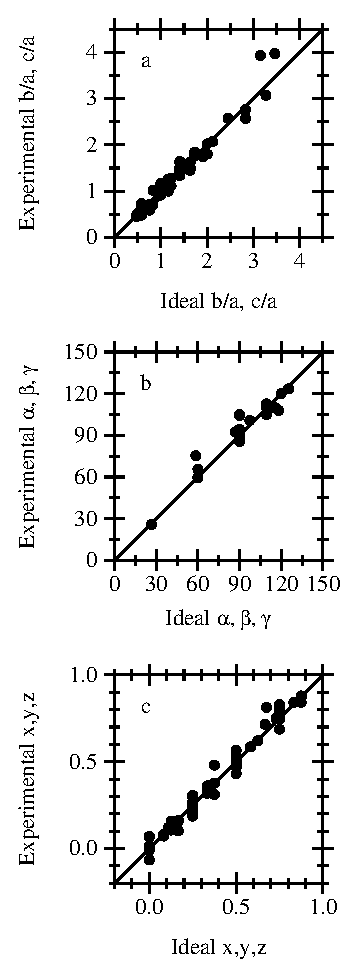
\includegraphics[width=\fullwidth]{compare2EPS.eps}
\end{center}
\caption[Comparison of experimental and ideal reference
structures.]{Comparison of experimental and ideal reference (a)
lattice lengths, (b) angles, and (c) structural parameters. The
45-degree line indicates perfect agreement between the experimental
molecular centers and the reference lattice. Scatter around the line
is the result of broken symmetry in orientationally ordered
structures.} \label{comparison}
\end{figure}

\begin{figure}
\begin{center}
\scalebox{.60}{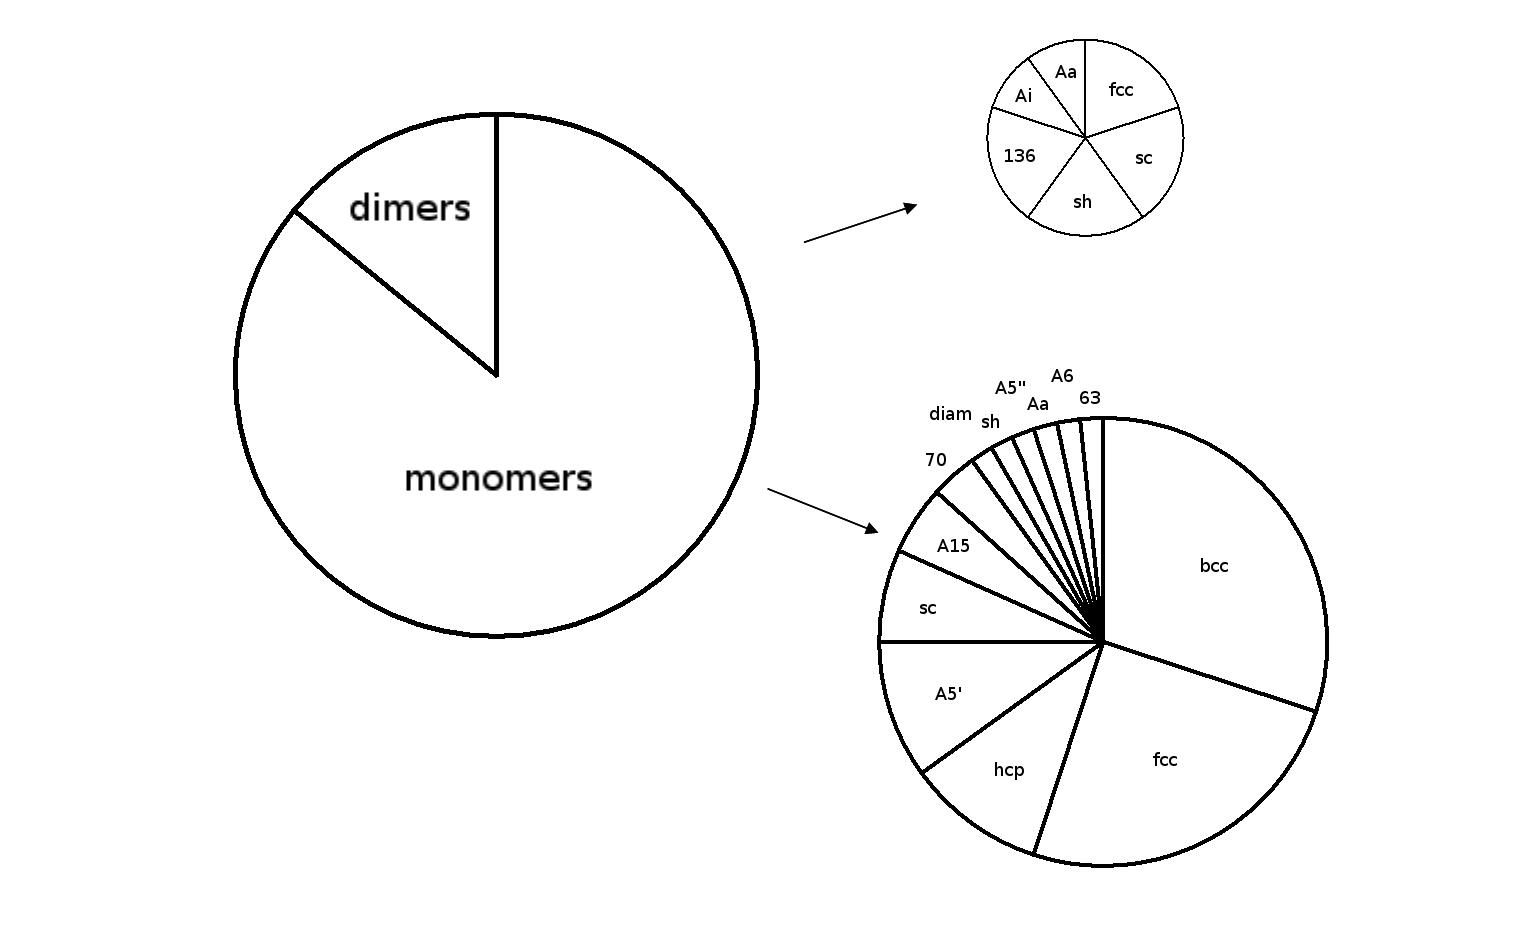
\includegraphics[width=\fullwidth]{pieCharts3.eps}}
\end{center}
\caption[Monomer and dimer structures and their reference
lattices.]{Relative proportions of monomer and dimer structures in
the experimental data set and reference lattices for
each.}\label{dimerMonomer}
\end{figure}

\begin{table}
\begin{center}
\caption{Dimer complexes among crystals of tetrahedral
molecules.}\label{tab:dimers}
\begin{tabular}{lccccc}
\hline
structure & dimer & representative & reference & point-group & entries\\
          &Wyck.~Pt.& entry        & lattice   & symmetry \\
\hline
205c & a & FOJBUB02 & d-fcc & $D_{3d}$              & 2\\
88f  & e & LUFYEQ   & d-Aa  & $C_{2v}$              & 1\\
14e  & a & TMSIAD   & d-sh  & $C_i$ ($\sim D_{3d}$) & 1 \\
14e  & a & CAMPOV   & d-sc  & $C_i$ ($\sim D_{3d}$) & 2\\
14e,e& e & CANFIG   & d-136 & $C_1$ ($\sim D_{3d}$) & 1\\
14e,e&b,c& MXSNOX   & d-sh  & $C_i$ ($\sim D_{3d}$) & 1\\
2i   & a & XAGXAE   & d-166 & $D_{3d}$              & 1\\
2i,i,i,i&i,i&CANFOM & d-136 & $C_1$ ($\sim D_{3d}$) & 1 \\
\cline{6-6}
\multicolumn{5}{r}{total:} & 10 \\
\hline \multicolumn{6}{c}{{\small Note: Point group symmetries were
assigned by visual inspection.}}
\end{tabular}
\end{center}
\end{table}


\end{document}
